\documentclass[12pt]{beamer}

\usetheme[progressbar=frametitle]{metropolis}
\usepackage{appendixnumberbeamer}

\usepackage{booktabs}
\usepackage[scale=2]{ccicons}

\usepackage{pgfplots}
\usepgfplotslibrary{dateplot}

\usepackage{xspace}
\newcommand{\themename}{\textbf{\textsc{metropolis}}\xspace}

\usepackage[UTF8]{ctex}
\usepackage{amsmath}
\usepackage{xcolor}
\usepackage{tikz}
\usepackage{amssymb}


\title{4.2.1 直线与圆的位置关系}
% \subtitle{等差数列的概念以及通项公式}
% \date{\today}
\date{}
\author{杨习}
\institute{shineyoung7@163.com}
% \titlegraphic{\hfill\includegraphics[height=1.5cm]{logo.pdf}}

\begin{document}

\maketitle

% \begin{frame}{主要知识点}
%   \setbeamertemplate{section in toc}[sections numbered]
%   \tableofcontents[hideallsubsections]
% \end{frame}

\begin{frame}\frametitle{知识回顾}
	\begin{description}[<+- | alert@+>]
		\item[点到直线的距离公式:] $ d=\frac{|Ax_0+By_0+C|}{\sqrt{A^2+B^2}} $
		\item[圆的标准方程:] $ (x-a)^2+(y-b)^2=r^2 (r>0) $
		\item[圆的一般方程:] $ x^2+y^2+Dx+Ey+F=0 $ \uncover<4,5,6>{\alert{$ (D^2+E^2-4F > 0) $}}\\
		\uncover<5,6>{圆心:\[(\alert{\frac{D}{-2}, \frac{E}{-2}})\]}\\
		\uncover<6>{半径:\[ r=\frac{\alert{\sqrt{D^2+E^2-4F}}}{2} \]}
	\end{description}
	\pause
\end{frame}

\section{直线与圆的位置关系}

\begin{frame}{线圆位置关系}
	圆心到直线的距离: $\alert{d}$, 圆的半径: $ \alert{r} $\vspace{20pt}

	\begin{columns}
		\column{0.5\textwidth}
			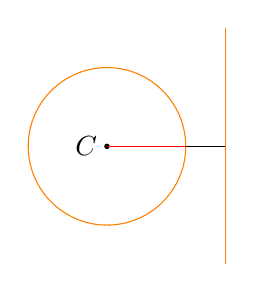
\begin{tikzpicture}
				\fill (0,0) circle [radius=1pt] node[left]{$C$};
				\draw[color=orange] (0,0) circle (1);
				\draw[color=orange] (1.5,1.5) -- (1.5,-1.5);
				\draw[color=black] (0,0)--(1.5,0);
				\draw[color=red] (0,0)--(1,0);
			\end{tikzpicture}
			\column{0.5\textwidth}
			\begin{itemize}[<+- | alert@+>]
				\item 相离
				\item $d>r$
				\item 没有交点
			\end{itemize}
	\end{columns}

 \end{frame}

 \begin{frame}{线圆位置关系}
		圆心到直线的距离: $\alert{d}$, 圆的半径: $ \alert{r} $\vspace{20pt}
		\begin{columns}
			\column{0.5\textwidth}
				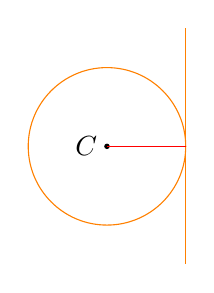
\begin{tikzpicture}
					\fill (0,0) circle [radius=1pt] node[left]{$C$};
					\draw[color=orange] (0,0) circle (1);
					\draw[color=orange] (1,1.5) -- (1,-1.5);
					\draw[color=black] (0,0)--(1,0);
					\draw[color=red] (0,0)--(1,0);
				\end{tikzpicture}
				\column{0.5\textwidth}
				\begin{itemize}[<+- | alert@+>]
					\item 相切
					\item $d=r$
					\item 有一个交点
				\end{itemize}
		\end{columns}
	\end{frame}

	\begin{frame}{线圆位置关系}
		圆心到直线的距离: $\alert{d}$, 圆的半径: $ \alert{r} $\vspace{20pt}
			\begin{columns}
				\column{0.5\textwidth}
				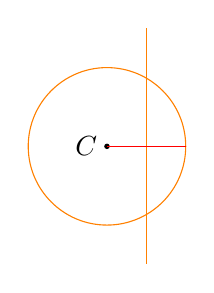
\begin{tikzpicture}
					\fill (0,0) circle [radius=1pt] node[left]{$C$};
					\draw[color=orange] (0,0) circle (1);
					\draw[color=orange] (0.5,1.5) -- (0.5,-1.5);
					\draw[color=black] (0,0)--(0.5,0);
					\draw[color=red] (0,0)--(1,0);
				\end{tikzpicture}
				\column{0.5\textwidth}
				\begin{itemize}[<+- | alert@+>]
					\item 相交
					\item $d<r$
					\item 有两个交点
				\end{itemize}
			\end{columns}

	\end{frame}

\section{直线与圆的位置关系 判定方法}

	\begin{frame}{几何法 判定}
		圆$ C: (x-\alert{a})^2+(y-\alert{b})^2=\alert{r}^2(r>0) $\\
		直线$ l: Ax+By+C=0 $ \vspace{20pt}

		1. 借助圆心到直线的\alert{距离$d$} 与\alert{半径$r$} 的大小关系进行判定:\vspace{22pt}

		\begin{columns}
			\column{0.5\textwidth}
			\begin{itemize}[<+- | alert@+>]
				\item $d>r$ $\Longleftrightarrow$ 相离
				\item $d=r$ $\Longleftrightarrow$ 相切
				\item $d<r$ $\Longleftrightarrow$ 相交
			\end{itemize}
			\column{0.5\textwidth}
			\uncover<4>{\[ d= \frac{|A\alert{a}+B\alert{b}+C|}{\sqrt{A^2+B^2}} \]}
		\end{columns}
	\end{frame}

	\begin{frame}{几何法判定——例题}
		\textcolor[rgb]{0.15,0.7,0.15}{例1.} 判断直线$l$与圆$C$的位置关系:\\
		圆$C: x^2+y^2-2x-24=0$\\
		直线$l: x+y-2=0$ \pause

		{\color{cyan} 解:由题知,
		圆心坐标为 $ (1,0) $, 圆的半径$r=5$\\ \pause
		则圆心到直圆心到直线的距离\[d=\frac{|1+0-2|}{\sqrt{1^2+1^2}} \pause \alert{< r} \]\\
		故直线与圆相交.
		}\pause

		\textcolor[rgb]{0.15,0.7,0.15}{练习1: }圆$C: x^2+y^2-2x-24=0$ \hspace{5pt}直线$l: 4x-3y+21=0$ \\\pause
		{\color{cyan} $d=5=r$ }
	\end{frame}

	\begin{frame}{代数法 判定}
		2. 借助直线与圆的公共点的个数进行判定:\vspace{22pt}
\begin{displaymath}
\left\{ \begin{array}{l}
(x-a)^2+(y-b)^2=r^2 \\
Ax+By+C=0
\end{array} \right.
\Longrightarrow
\textbf{关于$x(y)$的一元二次方程}
\end{displaymath}
则其\alert{解的个数}对应于\alert{线圆交点个数}
\begin{itemize}[<+- | alert@+>]
	\item $\Delta < 0$ $\Longleftrightarrow$ 没有交点 $\Longleftrightarrow$ 相离
	\item $\Delta = 0$ $\Longleftrightarrow$ 一个交点 $\Longleftrightarrow$ 相切
	\item $\Delta > 0$ $\Longleftrightarrow$ 两个交点 $\Longleftrightarrow$ 相交
\end{itemize}
	\end{frame}

	\begin{frame}{代数法 判定——例题}
		\textcolor[rgb]{0.15,0.7,0.15}{例2: }判断直线$l$与圆$C$的位置关系:\\
		圆$C: x^2+y^2=4$\\
		直线$l: y=2x+1$ \pause

		{\color{cyan} 解:由题知,
		联立方程组: \[\left\{ \begin{array}{l}
		x^2+y^2=4 \\
		y=2x+1
		\end{array} \right.\] \pause

		解得 $5x^2+4x-3=0$\\ \pause
		则其$\Delta = 76 > 0$\\ \pause
		故直线与圆相交.
		}\pause

		\textcolor[rgb]{0.15,0.7,0.15}{练习2: }圆$C: x^2+y^2-2x-1=0$\hspace{2pt}
		直线$l: x+y-2=0$\\ \pause
		{\color{cyan} $2x^2-6x+3=0$ \hspace{5pt}相交 }
	\end{frame}

	\begin{frame}{直线与圆的位置关系判定}
		\begin{itemize}[<+- | alert@+>]
			\item 相离 $\Longleftrightarrow$ $d>r$ $\Longleftrightarrow$ $\Delta < 0$
			\item 相切 $\Longleftrightarrow$ $d=r$ $\Longleftrightarrow$ $\Delta = 0$
			\item 相交 $\Longleftrightarrow$ $d<r$ $\Longleftrightarrow$ $\Delta > 0$
		\end{itemize}
	\end{frame}

	\begin{frame}{例题研究}
		\textcolor[rgb]{0.15,0.7,0.15}{例3: }若直线$ax+y=1$ 与圆$(x-1)^2+(y-2)^2=1$有两个不同的交点,则$a$的取值范围是\underline{\uncover<2,3>{\alert{$(-\infty,0)$}}}.\\\pause\vspace{10pt}

		\textcolor[rgb]{0.15,0.7,0.15}{练习3: }直线 $y=kx+2$ 与圆 $x^2+y^2=1$ 没有公共点,则 $k$ 的取值范围是\pause{\color{cyan} $(-\sqrt{3},\sqrt{3})$ }.
	\end{frame}

\begin{frame}{弦长问题}
	\textcolor[rgb]{0.15,0.7,0.15}{例4:}求直线$x-\sqrt{3}y+2\sqrt{3}=0$ 被圆$x^2+y^2=4$ 截得的弦长. \pause

	\vspace{20pt}

	\textcolor[rgb]{0.15,0.7,0.15}{例5: } 直线过点$(4,0)$, 且被圆$x^2+y^2-2x-2y-7=0$所截得的弦长最长,求直线的方程为.
\end{frame}
%
% \begin{frame}{弦长问题}
%
% \end{frame}

\begin{frame}{知识小结}
	1. 直线与圆的位置关系判定:
	\begin{description}[<+- | alert@+>]
		\item[相离] $\Longleftrightarrow$ $d>r$ $\Longleftrightarrow$ $\Delta < 0$
		\item[相切] $\Longleftrightarrow$ $d=r$ $\Longleftrightarrow$ $\Delta = 0$
		\item[相交] $\Longleftrightarrow$ $d<r$ $\Longleftrightarrow$ $\Delta > 0$
	\end{description}\pause
	圆心到直线的距离\[ d= \frac{|A\alert{a}+B\alert{b}+C|}{\sqrt{A^2+B^2}} \]\pause
	\[\left\{ \begin{array}{l}
	(x-a)^2+(y-b)^2=r^2 \\
	Ax+By+C=0
	\end{array} \right.
	\Longrightarrow
	\textbf{关于$x(y)$的一元二次方程}\]
	\textbf{\alert{判别式$\Delta$}}
\end{frame}

\begin{frame}{课后作业}
	《课时作业(二十八)》
\end{frame}


% \section{生活中的等差数列}
%
% 	\begin{frame}[fragile]\frametitle{生活中的等差数列}
%
% 		姚明刚进NBA一周里训练罚球的个数:
% 		\begin{columns}
% 			\column{0.8\textwidth}
% 				\begin{itemize}[<+- | +->]
% 					\item 第一天:6000
% 					\item 第二天:6500
% 					\item 第三天:7000
% 					\item 第四天:7500
% 					\item 第五天:8000
% 					\item 第六天:8500
% 					\item 第七天:9000
% 					\item \textbf{得到数列:}6000, 6500, 7000, 7500, 8000, 8500, 9000
% 				\end{itemize}
% 			\column{0.2\textwidth}
% 				
\includegraphics[width=\textwidth]{ap2.jpg}
% 		\end{columns}
%
% 	\end{frame}
%
% 	\begin{frame}[fragile]\frametitle{生活中的等差数列}
%
% 		女式运动鞋的尺码数:
% 		\begin{columns}
% 			\column{0.8\textwidth}
% 				\begin{itemize}[<+- | +->]
% 					\item 22
% 					\item 22.5
% 					\item 23
% 					\item 23.5
% 					\item 24
% 					\item 24.5
% 					\item 25
% 					\item \textbf{得到数列:}22, 22.5, 23, 23.5, 24, 24.5, 25
% 				\end{itemize}
% 			\column{0.2\textwidth}
% 				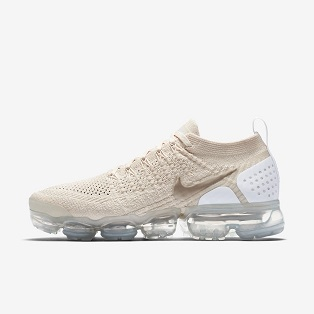
\includegraphics[width=\textwidth]{ap3.jpg}
% 		\end{columns}
%
% 	\end{frame}
%
% 	\begin{frame}[fragile]\frametitle{生活中的等差数列}
%
% 		哈雷彗星的回归年份:
% 		\begin{columns}
% 			\column{0.6\textwidth}
% 				\begin{itemize}[<+- | +->]
% 					\item 1682
% 					\item 1758
% 					\item 1834
% 					\item 1910
% 					\item 1986
% 					\item 2062
% 					\item \textbf{得到数列:}1682, 1758, 1834, 1910, 1986, 2062
% 				\end{itemize}
% 			\column{0.4\textwidth}
% 				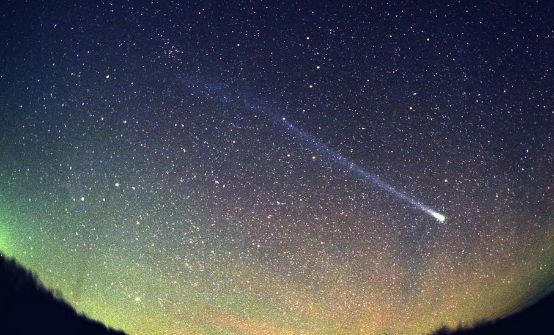
\includegraphics[width=\textwidth]{ap1.jpg}
% 		\end{columns}
%
% 	\end{frame}
%
% 	\begin{frame}{生活中的等差数列}
% 		\begin{itemize}
% 			\item[*] 6000, 6500, 7000, 7500, 8000, 8500, 9000 \vspace{15pt}
% 			\item[*] 22, 22.5, 23, 23.5, 24, 24.5, 25 \vspace{15pt}
% 			\item[*] 1682, 1758, 1834, 1910, 1986, 2062
% 		\end{itemize}
% 		\pause
% 		\begin{itemize}[<+->]
% 			\item \textbf{观察:} 以上数列有什么共同特点?
% 			\item \alert{从第2项起}, 每一项与前一项的差都等于\alert{同一常数}
% 		\end{itemize}
% 	\end{frame}
%
% \section{等差数列的概念}
% 	\subsection{等差数列的定义}
% 		\begin{frame}\frametitle{等差数列的定义}
%
% 			一般地,如果一个数列从\alert{\textbf{第2项起}},每一项与它的前一项的差等于\alert{\textbf{同一个常数}},那么这个数列就叫做等差数列.
% 			\pause
%
% 			这个常数叫做等差数列的\alert{公差},通常用字母\alert{$d$}表示。
%
% 		\end{frame}
%
% 	\subsection{小测验判断是否为等差数列}
% 		\begin{frame}\frametitle{等差数列的定义}
%
% 			小测验:判断下列数列是否为等差数列,如果是,求出公差
% 			\pause
% 			\begin{enumerate}[<+->]
% 				\item 数列4, 7, 10, 13, 16, $\ldots$; \hspace{10pt}\uncover<6,7,8,9,10>{公差是3}
% 				\item 数列6, 4, 2, 0, -2, -4; \hspace{10pt}\uncover<7,8,9,10>{公差是-2}
% 				\item 数列 1, 1, 1, 1, 1; \hspace{10pt}\uncover<8,9,10>{公差是0}
% 				\item 数列 -3, -2, -1, 1, 2, 3. \hspace{10pt}\uncover<9,10>{不是}
% 			\end{enumerate}
% 			\pause
% 			\pause
% 			\pause
% 			\pause
% 			\metroset{block=fill}
% 			\begin{alertblock}{注意:}
% 				公差$d$是每一项(第2项起)与它的前一项的差,而且公差可以是正数,负数,也可以为0.
% 			\end{alertblock}
%
% 		\end{frame}
%
% 		\begin{frame}\frametitle{公差$d$ 取不同值时数列特点}
%
% 			设等差数列$\{a_n\}$的公差为$d$:
% 			\pause
% 			\begin{description}[<+- | alert@+>]
% 				\item[$d>0$时,] $\{a_n\}$为递增数列;
% 				\item[$d<0$时,] $\{a_n\}$为递减数列;
% 				\item[$d=0$时,] $\{a_n\}$为常数列.
% 			\end{description}
% 			\pause
%
% 		\end{frame}
%
% 		\begin{frame}\frametitle{等差数列的定义}
%
% 			一般地,如果一个数列从\pause \alert{\textbf{第2项起}}, \pause 每一项与它的前一项的差等于\pause \alert{\textbf{同一个常数$d$}}, \pause 那么这个数列就叫做等差数列.
% 			\pause
%
% 			\begin{large}
% 				\[ \mathbf{a_n-a_{n-1}=d}\quad \pause (n\geq 2, n\in \mathbf{N_+} ) \] \pause 或
% 				\[ \mathbf{a_{n+1}-a_n=d}  \pause \quad (n\in \mathbf{N_+}) \]
% 			\end{large}
%
% 		\end{frame}
%
%
% \section{等差数列的通项公式}
% 	\subsection{通项公式推导}
%
% 		% \begin{frame}\frametitle{等差数列的通项公式推导}
%
% 		% 	观察数列:-1,1,3,5,7, $\ldots$\\ \pause
% 		% 	$a_{100}={\color{red}?}$
%
% 		% \end{frame}
%
% 		\begin{frame}\frametitle{等差数列的通项公式 推导}
%
% 			如果一个数列$\{a_n\}$是等差数列, 首项是$a_1$, 公差是$d$,则这个数列的通项公式是什么呢?\pause
%
% 				$a_2=a_1+d$\\ \pause
% 				$a_3=a_2+d=a_1+2d$\\ \pause
% 				$a_4=a_3+d=a_1+3d$\\ \pause
% 				$a_5=a_4+d=a_1+4d$\\ \pause
% 				$\hspace{2pt}\vdots \hspace{26pt} \vdots$\\
% 				$a_n=\only<6>{\color{red}?} \only<7>{\alert{a_1+(n-1)d}}$
%
% 		\end{frame}
%
% 		\begin{frame}\frametitle{等差数列的通项公式 推导}
%
% 			问:是否还有其他办法来推导等差数列的通项公式?\pause
% 			\vspace{10pt}
%
% 			\begin{columns}
% 				\column{0.5\textwidth}
% 				根据等差数列的定义: \pause
% 				$a_2-a_1{\color{cyan}=}d$\\ \pause
% 				$a_3-a_2{\color{cyan}=}d$\\ \pause
% 				$a_4-a_3{\color{cyan}=}d$\\ \pause
% 				$a_5-a_4{\color{cyan}=}d$\\ \pause
% 				$\hspace{2pt}\vdots \hspace{26pt} \vdots$\\
% 				$a_n-a_{n-1}{\color{cyan}=}d$\\ \pause
% 				\vspace{10pt}
% 				$a_n-a_1=\only<8>{\color{red}?} \only<9,10,11,12>{\alert{(n-1)d}}$
% 				\pause
%
% 				\pause
% 				\column{0.5\textwidth}
%
% 				由此我们得到:
% 				\metroset{block=fill}
% 				\begin{block}{等差数列的通项公式}
% 					${\color{red}a_n=a_1+(n-1)d}$
% 				\end{block}
%
% 				% \begin{block}{通项公式 推广式}
% 				%  	${\color{red}a_n=a_m+(n-m)d}$\\ \vspace{10pt} \pause
% 				%  	变形式: \[d=\frac{a_n-a_m}{n-m}\]
% 				% \end{block}
% 			\end{columns}
% 		\end{frame}
%
%
% 	\subsection{通项公式定义}
% 		\begin{frame}\frametitle{等差数列的通项公式}
%
% 			若一个等差数列$\{a_n\}$, 它的首项为$a_1$, 公差是$d$, 那么这个数列的通项公式是: \pause
% 			\[ \mathbf{\alert{a_n=a_1+(n-1)d}} \]
%
% 			\pause
% 			\begin{columns}
% 				\column{0.5\textwidth}
% 				其中涉及到的独立的量有: \pause
% 				\begin{itemize}[<+-|alert@+>]
% 					\item $a_n$
% 					\item $a_1$
% 					\item $n$
% 					\item $d$
% 				\end{itemize}
%
% 				\pause
% 				\column{0.5\textwidth}
% 				{\color{magenta} 知三求一}
% 			\end{columns}
%
% 		\end{frame}
%
% 	\subsection{题型研究}
% 		\begin{frame}\frametitle{通项公式题型研究 \hspace{40pt} \alert{$a_n=a_1+(n-1)d$}}
%
% 		\begin{block}{题型一: 求通项$a_n$}\pause
% 			\textcolor[rgb]{0.15,0.7,0.15}{例1.} (1) $a_1=1, d=2, n=10$, 求$a_{10}=?$\\ \pause
% 			{\color{cyan} 解: $a_{10}=a_1+9d \pause =19$}\\
% 			\pause
% 			$a_n=\only<5>{\color{red}?}\pause 1+(n-1)\cdot2 \pause =2n-1$ \pause
%
% 			(2) 已知等差数列$8, 5, 2, \ldots$ 求$a_n$及$a_{20}$. \\ \pause
% 			{\color{cyan} 解: 由题知, \\ $a_1=8$\\ \pause
% 			$d=5-8=-3$\\ \pause
% 			$\therefore a_n=8+(n-1)\cdot(-3) \pause =-3n+11$\\ \pause
% 			$\therefore a_{20}=-49$
% 			}
% 			\pause
%
% 			\textcolor[rgb]{0.15,0.7,0.15}{练习1: } 已知等差数列$3, 7, 11, \ldots$, 则\\ \pause
% 			$a_n=\pause 4n-1$ \hspace{30pt} \pause
% 			$a_4=\pause 15$ \hspace{30pt} \pause
% 			$a_{10}=\pause 39$
%
% 		\end{block}
%
% 		\end{frame}
%
% 		\begin{frame}\frametitle{通项公式题型研究 \hspace{40pt} \alert{$a_n=a_1+(n-1)d$}}
%
% 		\begin{block}{题型二: 求首项$a_1$}\pause
% 			\textcolor[rgb]{0.15,0.7,0.15}{例2.} 已知等差数列$\{a_n\}$中, $a_{20}=-49, d=-3$, 求首项$a_1$. \pause
% 			{\color{cyan} 解: 由$a_{20}=a_1+19d$ \\ \pause
% 			得$a_1=8$}
% 			\pause
%
% 			\textcolor[rgb]{0.15,0.7,0.15}{练习2: } $a_4=15, d=3, 则a_1=\only<5>{\color{red}?}\pause 6$
%
% 		\end{block}
%
% 		\end{frame}
%
% 		\begin{frame}\frametitle{通项公式题型研究 \hspace{40pt} \alert{$a_n=a_1+(n-1)d$}}
%
% 		\begin{block}{题型三: 求项数$n$}\pause
% 			\textcolor[rgb]{0.15,0.7,0.15}{例3.} 判断$-400$是不是等差数列$-5, -9, -13, \ldots$的项?如果是, 是第几项? \\ \pause
% 			{\color{cyan} 解: $a_1=-5$, \pause $d=-4$, \pause $a_n=-5+(n-1)\cdot(-4)$\\ \pause
% 			假设 $-400$是该等差数列中的第$n$项, \\ \pause
% 			则 $-400=-5+(n-1)\cdot(-4)$ \\ \pause
% 			解之得, $n=\frac{399}{4} \hspace{20pt}$(不是正整数) \\ \pause
% 			所以$-400$不是这个数列的项.
% 			}
% 			\pause
%
% 			\textcolor[rgb]{0.15,0.7,0.15}{练习3: } $100$是不是等差数列$2, 9, 16, \ldots$的项? 如果是, 是第几项? 如果不是, 说明理由. \\ \pause
% 			{\color{cyan} 是, 第15项}
% 		\end{block}
%
% 		\end{frame}
%
%
%
% 		\begin{frame}\frametitle{通项公式题型研究 \hspace{40pt} \alert{$a_n=a_1+(n-1)d$}}
%
% 		\begin{block}{题型四: 列方程组求基本量}\pause
% 			\textcolor[rgb]{0.15,0.7,0.15}{例4.} 在等差数列中,已知$a_5=10, a_{12}=31$, 求首项$a_1$与公差$d$. \\ \pause
%
% 			{\color{cyan} 解: 由题意知\\
% 			\[ \left\{
% 				\begin{array}{l}
% 					10=a_1+4d\\
% 					31=a_1+11d
% 				\end{array}
% 				\right. \] \pause
%
% 			解方程组得:\\
% 			\[ \left\{
% 				\begin{array}{l}
% 					a_1=-2\\
% 					d=3
% 				\end{array}
% 				\right. \]
% 			}
%
% 		\end{block}
%
% 		\end{frame}
%


		% \begin{frame}\frametitle{通项公式题型研究 \hspace{40pt} \alert{$a_n=a_1+(n-1)d$}}

		% \begin{block}{题型四: 求公差$d$}\pause
		% 	\textcolor[rgb]{0.15,0.7,0.15}{例4.} 一张梯子最高一级宽$33cm$, 最低一级宽$110cm$, 中间还有$10$级, 各级的宽度成等差数列. 求公差$d$及中间各级的宽度. \\ \pause
		% 	{\color{orange} 提示: 用$\{a_n\}$表示梯子自上而下各级宽度所成的等差数列.
		% 	}
		% 	\pause

		% 	{\color{cyan} 解: 由题意知, $a_1=33, a_{12}=110, n=12$\\ \pause
		% 	$\therefore 110=33+(12-1)d$\\ \pause
		% 	解得 $d=7$\\ \pause
		% 	$\therefore a_2=33+7=40$\\ \pause
		% 	$a_3=40+7=47$\\ \pause
		% 	$a_4=47+7=54$ $\ldots$
		% 	}
		% 	\pause

		% \end{block}

		% \end{frame}


% 		\subsection{等差中项}
% 		\begin{frame}\frametitle{等差中项}

% 			问:如果在$a$与$b$中间插入一个数$A$,使$a, A, b$成等差数列,那么A应满足什么条件?

% 			\pause
% 			因为$a, A, b$组成了一个等差数列,那么由定义可以知道: \[\alert{A-a=b-A}\]
% 			\pause
% 			即 \[ A=\frac{a+b}{2} \]
% 			\pause
% 			\metroset{block=fill}
% 			\begin{exampleblock}{小练习}
% 				(1)\hspace{2pt} 2, \uncover<5,6>{\alert{5}}, 8; \\
% 			(2)\hspace{2pt} $\sqrt{3}-1, $ \uncover<6>{\alert{$\sqrt{3}$}}, $\sqrt{3}+1$
% 			\end{exampleblock}

% 		\end{frame}

% 		\begin{frame}\frametitle{等差中项}
% 		    \metroset{block=fill}
% 			\begin{block}{等差中项的定义}
% 			如果$a, \alert{A}, b$组成了一个等差数列,那么$\alert{A}$叫做$a$与$b$的\\等差中项.
% 			\end{block}
% 			\pause

% 			\textcolor[rgb]{0.15,0.7,0.15}{例5.}已知$a=\frac{1}{\sqrt{3}+\sqrt{2}}, b=\frac{1}{\sqrt{3}-\sqrt{2}}$求$a, b$的等差中项.
% 			\pause
% 			\vspace{7pt}

% 				{\color{cyan} 解: 设$a, b$的等差中项为$A$, 则 \pause
% 				\[ A=\frac{a+b}{2} \pause =\frac{\frac{1}{\sqrt{3}+\sqrt{2}}+\frac{1}{\sqrt{3}-\sqrt{2}}}{2} \pause =\frac{\frac{\sqrt{3}-\sqrt{2}}{3-2}+\frac{\sqrt{3}+\sqrt{2}}{3-2}}{2} \pause =\sqrt{3} \]}

% 			\textcolor[rgb]{0.15,0.7,0.15}{练习4: } 三角形的三个内角$A, B, C$成等差数列,求角$B$.

% 		\end{frame}



% \section{与一次函数图象的类比探究}

% 	\begin{frame}\frametitle{类比探究一次函数}

% 		已知在等差数列$\{a_n\}$中, $a_1=-2$, $d=2$, 求通项公式$a_n$. \vspace{20pt}\pause

% 		\begin{columns}
% 			\column{0.5\textwidth}
% 			并在直角坐标系中画出它的图象, 观察图像有什么特点? \pause \vspace{32pt}

% 			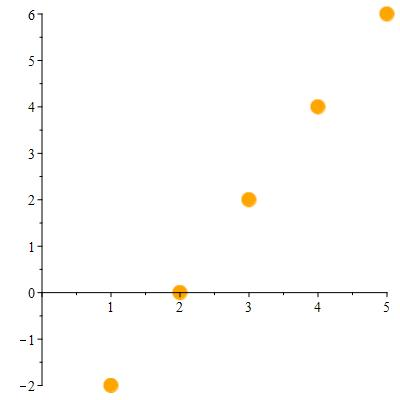
\includegraphics[width=0.77\textwidth]{ap4.jpg} \pause

% 			\column{0.5\textwidth}
% 			在同一个直角坐标系中, 画出函数$\alert{y=2x-4}$的图像,观察与数列$\alert{a_n=2n-4}$的图像有什么关系? \pause

% 			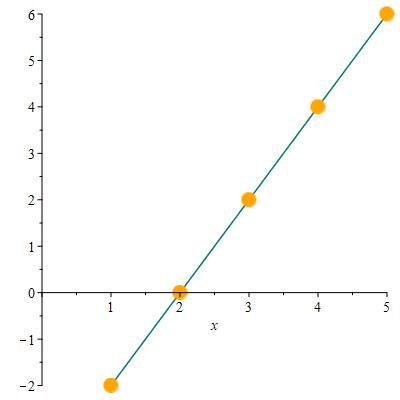
\includegraphics[width=0.77\textwidth]{ap5.jpg}

% 		\end{columns}



% 	\end{frame}
%
% \section{知识回顾}
%
% 	\begin{frame}\frametitle{课堂小结}
%
% 		\begin{description}[<+-|alert@+>]
% 			\item[一个定义] $a_{n+1}-a_n=d$
% 			\item[一个方法] 累加法
% 			\item[一个公式] $a_n=a_1+(n-1)d$
% 			\item[一个思想] 方程思想
% 		\end{description}
%
% 	\end{frame}
%
% 	\begin{frame}\frametitle{课后作业}
%
% 		《教材》 40页 习题2.2 \\
% 		A组 1,3,4\\
% 		B组 2
% 		\vspace{30pt}
%
% 		探究性作业:\\
% 		在自己身边找出一个等差数列的例子,找出它的首项、公差.
%
% 	\end{frame}

% \begin{frame}[fragile]{Metropolis}

%   The \themename theme is a Beamer theme with minimal visual noise
%   inspired by the \href{https://github.com/hsrmbeamertheme/hsrmbeamertheme}{\textsc{hsrm} Beamer
%   Theme} by Benjamin Weiss.

%   Enable the theme by loading

%   \begin{verbatim}    \documentclass{beamer}
%     \usetheme{metropolis}\end{verbatim}

%   Note, that you have to have Mozilla's \emph{Fira Sans} font and XeTeX
%   installed to enjoy this wonderful typography.
% \end{frame}
% \begin{frame}[fragile]{Sections}
%   Sections group slides of the same topic

%   \begin{verbatim}    \section{Elements}\end{verbatim}

%   for which \themename provides a nice progress indicator \ldots
% \end{frame}

% \section{Titleformats}

% \begin{frame}{Metropolis titleformats}
% 	\themename supports 4 different titleformats:
% 	\begin{itemize}
% 		\item Regular
% 		\item \textsc{Smallcaps}
% 		\item \textsc{allsmallcaps}
% 		\item ALLCAPS
% 	\end{itemize}
% 	They can either be set at once for every title type or individually.
% \end{frame}

% {
%     \metroset{titleformat frame=smallcaps}
% \begin{frame}{Small caps}
% 	This frame uses the \texttt{smallcaps} titleformat.

% 	\begin{alertblock}{Potential Problems}
% 		Be aware, that not every font supports small caps. If for example you typeset your presentation with pdfTeX and the Computer Modern Sans Serif font, every text in smallcaps will be typeset with the Computer Modern Serif font instead.
% 	\end{alertblock}
% \end{frame}
% }

% {
% \metroset{titleformat frame=allsmallcaps}
% \begin{frame}{All small caps}
% 	This frame uses the \texttt{allsmallcaps} titleformat.

% 	\begin{alertblock}{Potential problems}
% 		As this titleformat also uses smallcaps you face the same problems as with the \texttt{smallcaps} titleformat. Additionally this format can cause some other problems. Please refer to the documentation if you consider using it.

% 		As a rule of thumb: Just use it for plaintext-only titles.
% 	\end{alertblock}
% \end{frame}
% }

% {
% \metroset{titleformat frame=allcaps}
% \begin{frame}{All caps}
% 	This frame uses the \texttt{allcaps} titleformat.

% 	\begin{alertblock}{Potential Problems}
% 		This titleformat is not as problematic as the \texttt{allsmallcaps} format, but basically suffers from the same deficiencies. So please have a look at the documentation if you want to use it.
% 	\end{alertblock}
% \end{frame}
% }

% \section{Elements}

% \begin{frame}[fragile]{Typography}
%       \begin{verbatim}The theme provides sensible defaults to
% \emph{emphasize} text, \alert{accent} parts
% or show \textbf{bold} results.\end{verbatim}

%   \begin{center}becomes\end{center}

%   The theme provides sensible defaults to \emph{emphasize} text,
%   \alert{accent} parts or show \textbf{bold} results.
% \end{frame}

% \begin{frame}{Font feature test}
%   \begin{itemize}
%     \item Regular
%     \item \textit{Italic}
%     \item \textsc{SmallCaps}
%     \item \textbf{Bold}
%     \item \textbf{\textit{Bold Italic}}
%     \item \textbf{\textsc{Bold SmallCaps}}
%     \item \texttt{Monospace}
%     \item \texttt{\textit{Monospace Italic}}
%     \item \texttt{\textbf{Monospace Bold}}
%     \item \texttt{\textbf{\textit{Monospace Bold Italic}}}
%   \end{itemize}
% \end{frame}

% \begin{frame}{Lists}
%   \begin{columns}[T,onlytextwidth]
%     \column{0.33\textwidth}
%       Items
%       \begin{itemize}
%         \item Milk \item Eggs \item Potatos
%       \end{itemize}

%     \column{0.33\textwidth}
%       Enumerations
%       \begin{enumerate}
%         \item First, \item Second and \item Last.
%       \end{enumerate}

%     \column{0.33\textwidth}
%       Descriptions
%       \begin{description}
%         \item[PowerPoint] Meeh. \item[Beamer] Yeeeha.
%       \end{description}
%   \end{columns}
% \end{frame}
% \begin{frame}{Animation}
%   \begin{itemize}[<+- | alert@+>]
%     \item \alert<4>{This is\only<4>{ really} important}
%     \item Now this
%     \item And now this
%   \end{itemize}
% \end{frame}
% \begin{frame}{Figures}
%   \begin{figure}
%     \newcounter{density}
%     \setcounter{density}{20}
%     \begin{tikzpicture}
%       \def\couleur{alerted text.fg}
%       \path[coordinate] (0,0)  coordinate(A)
%                   ++( 90:5cm) coordinate(B)
%                   ++(0:5cm) coordinate(C)
%                   ++(-90:5cm) coordinate(D);
%       \draw[fill=\couleur!\thedensity] (A) -- (B) -- (C) --(D) -- cycle;
%       \foreach \x in {1,...,40}{%
%           \pgfmathsetcounter{density}{\thedensity+20}
%           \setcounter{density}{\thedensity}
%           \path[coordinate] coordinate(X) at (A){};
%           \path[coordinate] (A) -- (B) coordinate[pos=.10](A)
%                               -- (C) coordinate[pos=.10](B)
%                               -- (D) coordinate[pos=.10](C)
%                               -- (X) coordinate[pos=.10](D);
%           \draw[fill=\couleur!\thedensity] (A)--(B)--(C)-- (D) -- cycle;
%       }
%     \end{tikzpicture}
%     \caption{Rotated square from
%     \href{http://www.texample.net/tikz/examples/rotated-polygons/}{texample.net}.}
%   \end{figure}
% \end{frame}
% \begin{frame}{Tables}
%   \begin{table}
%     \caption{Largest cities in the world (source: Wikipedia)}
%     \begin{tabular}{lr}
%       \toprule
%       City & Population\\
%       \midrule
%       Mexico City & 20,116,842\\
%       Shanghai & 19,210,000\\
%       Peking & 15,796,450\\
%       Istanbul & 14,160,467\\
%       \bottomrule
%     \end{tabular}
%   \end{table}
% \end{frame}
% \begin{frame}{Blocks}
%   Three different block environments are pre-defined and may be styled with an
%   optional background color.

%   \begin{columns}[T,onlytextwidth]
%     \column{0.5\textwidth}
%       \begin{block}{Default}
%         Block content.
%       \end{block}

%       \begin{alertblock}{Alert}
%         Block content.
%       \end{alertblock}

%       \begin{exampleblock}{Example}
%         Block content.
%       \end{exampleblock}

%     \column{0.5\textwidth}

%       \metroset{block=fill}

%       \begin{block}{Default}
%         Block content.
%       \end{block}

%       \begin{alertblock}{Alert}
%         Block content.
%       \end{alertblock}

%       \begin{exampleblock}{Example}
%         Block content.
%       \end{exampleblock}

%   \end{columns}
% \end{frame}
% \begin{frame}{Math}
%   \begin{equation*}
%     e = \lim_{n\to \infty} \left(1 + \frac{1}{n}\right)^n
%   \end{equation*}
% \end{frame}
% \begin{frame}{Line plots}
%   \begin{figure}
%     \begin{tikzpicture}
%       \begin{axis}[
%         mlineplot,
%         width=0.9\textwidth,
%         height=6cm,
%       ]

%         \addplot {sin(deg(x))};
%         \addplot+[samples=100] {sin(deg(2*x))};

%       \end{axis}
%     \end{tikzpicture}
%   \end{figure}
% \end{frame}
% \begin{frame}{Bar charts}
%   \begin{figure}
%     \begin{tikzpicture}
%       \begin{axis}[
%         mbarplot,
%         xlabel={Foo},
%         ylabel={Bar},
%         width=0.9\textwidth,
%         height=6cm,
%       ]

%       \addplot plot coordinates {(1, 20) (2, 25) (3, 22.4) (4, 12.4)};
%       \addplot plot coordinates {(1, 18) (2, 24) (3, 23.5) (4, 13.2)};
%       \addplot plot coordinates {(1, 10) (2, 19) (3, 25) (4, 15.2)};

%       \legend{lorem, ipsum, dolor}

%       \end{axis}
%     \end{tikzpicture}
%   \end{figure}
% \end{frame}
% \begin{frame}{Quotes}
%   \begin{quote}
%     Veni, Vidi, Vici
%   \end{quote}
% \end{frame}

% {%
% \setbeamertemplate{frame footer}{My custom footer}
% \begin{frame}[fragile]{Frame footer}
%     \themename defines a custom beamer template to add a text to the footer. It can be set via
%     \begin{verbatim}\setbeamertemplate{frame footer}{My custom footer}\end{verbatim}
% \end{frame}
% }

% \begin{frame}{References}
%   Some references to showcase [allowframebreaks] \cite{knuth92,ConcreteMath,Simpson,Er01,greenwade93}
% \end{frame}

% \section{Conclusion}

% \begin{frame}{Summary}

%   Get the source of this theme and the demo presentation from

%   \begin{center}\url{github.com/matze/mtheme}\end{center}

%   The theme \emph{itself} is licensed under a
%   \href{http://creativecommons.org/licenses/by-sa/4.0/}{Creative Commons
%   Attribution-ShareAlike 4.0 International License}.

%   \begin{center}\ccbysa\end{center}

% \end{frame}

% {\setbeamercolor{palette primary}{fg=black, bg=orange}
% \begin{frame}[standout]
%   Questions?
% \end{frame}
% }

% \appendix

% \begin{frame}[fragile]{Backup slides}
%   Sometimes, it is useful to add slides at the end of your presentation to
%   refer to during audience questions.

%   The best way to do this is to include the \verb|appendixnumberbeamer|
%   package in your preamble and call \verb|\appendix| before your backup slides.

%   \themename will automatically turn off slide numbering and progress bars for
%   slides in the appendix.
% \end{frame}

% \begin{frame}[allowframebreaks]{References}

%   \bibliography{demo}
%   \bibliographystyle{abbrv}

% \end{frame}

\end{document}
